% Astronomía para Todos - Taller de ejercicios sobre magnitudes (puntos 1 a 5)
% Compilar desde esta carpeta:  tectonic taller_magnitudes.tex
\documentclass[11pt,a4paper]{article}

\usepackage[spanish,es-nodecimaldot,es-tabla]{babel}
\usepackage{fontspec}
\usepackage{amsmath}
\usepackage{siunitx}
\usepackage{booktabs}
\usepackage{graphicx}
\usepackage{float}
\usepackage[font=small,labelfont=bf]{caption}
\usepackage[margin=2.4cm]{geometry}
\usepackage{microtype}
\usepackage[hidelinks]{hyperref}

\sisetup{output-decimal-marker={.}, group-separator={\,}, group-minimum-digits=4}
\graphicspath{{../resultados/}}

% Nombre del estudiante: reemplazar antes de entregar.
\newcommand{\autor}{Nombre del estudiante}

\title{Astronomía para Todos\\[4pt]\large Taller de ejercicios sobre magnitudes: puntos 1 a 5}
\author{\autor}
\date{29 de octubre de 2026}

\begin{document}
\maketitle

\begin{abstract}
Se resuelven los cinco puntos del taller. Los puntos 1 a 3 son cálculos con paralajes y
magnitudes. El punto 4 estudia la Gran Nube de Magallanes (LMC) en óptico, infrarrojo, radio y
rayos gamma: se mide su diámetro angular en cada banda con dos métodos y se construye el diagrama
color-magnitud de 1100 estrellas masivas del catálogo de Bonanos et al.\ (2009). El punto 5 estima la
edad del cúmulo abierto NGC~4755 (la Caja de Joyas) a partir de la foto del taller, y la contrasta
con un diagrama color-magnitud real de Gaia~DR3 y con la literatura. Los servidores del CDS
(Estrasburgo) no respondieron durante todo el trabajo, por lo que se usaron fuentes alternativas,
detalladas en el apéndice~\ref{ap:fuentes}.
\end{abstract}

\tableofcontents

% =====================================================================
\section{Punto 1: un tren a $\alpha$~Centauri}

\textbf{Datos.} Velocidad $v = \SI{100}{km/h}$; paralaje de $\alpha$~Cen $p = 0.760''$.
Constantes: $\SI{1}{pc} = \SI{3.0857e13}{km} = \num{3.2616}$ años luz; 1 año $= \SI{8766}{h}$.

Con la paralaje en segundos de arco, la distancia en parsecs es $d = 1/p$:
\begin{align}
d &= \frac{1}{0.760} = \SI{1.316}{pc} = 1.316 \times \SI{3.0857e13}{km} = \SI{4.060e13}{km}
\quad (\approx 4.29 \text{ años luz}),\\
t &= \frac{d}{v} = \frac{\SI{4.060e13}{km}}{\SI{100}{km/h}} = \SI{4.060e11}{h}
= \frac{\SI{4.060e11}{h}}{\SI{8766}{h/año}} = \num{4.63e7}\ \text{años}.
\end{align}

\textbf{Respuesta: unos 46 millones de años.} Como comparación, hace 46 millones de años ya se
habían extinguido los dinosaurios no avianos (hace 66 millones de años), pero todavía no existían
los homínidos. Con la paralaje actual de SIMBAD para el sistema ($750.8$~mas) el viaje duraría
$\num{4.69e7}$ años: la conclusión no cambia.

% =====================================================================
\section{Punto 2: ¿Venus de día desde el fondo de un pozo?}

\textbf{Datos.} El ojo distingue un contraste del 5\,\%; el cielo diurno tiene magnitud aparente
$m_\text{cielo} = -5.2$.

\subsection{Criterio de brillo}
Para distinguir Venus, su flujo debe ser al menos el 5\,\% del flujo del cielo de fondo. Como
$m_1 - m_2 = -2.5\log_{10}(F_1/F_2)$, el objeto más débil detectable tiene
\begin{equation}
m_\text{lím} = m_\text{cielo} + 2.5\log_{10}\!\left(\frac{1}{0.05}\right) = -5.2 + 3.25 = -1.95 .
\end{equation}
En su máximo brillo Venus llega a magnitud $-4.4$ a $-4.6$ \cite{naoj,earthsky}, y su razón de flujos
con el cielo es
\begin{equation}
\frac{F_\text{Venus}}{F_\text{cielo}} = 10^{-0.4\,(-4.6+5.2)} = 10^{-0.24} = 0.58
\qquad (0.48 \text{ con } m = -4.4),
\end{equation}
unas diez veces más que el 5\,\% necesario. \textbf{Por brillo, Venus sí se puede ver de día.}

\subsection{El papel del pozo}
\begin{itemize}
  \item \textbf{El pozo no oscurece el cielo.} Las paredes tapan la mayor parte del cielo, pero el
  trozo visible tiene el mismo brillo por unidad de área. El contraste es el mismo que fuera del
  pozo; que desde un pozo se vean estrellas de día es un mito.
  \item \textbf{Sí limita hacia dónde se mira.} Desde el fondo solo se ve una zona pequeña alrededor
  del cenit: un pozo de \SI{1}{m} de diámetro y \SI{20}{m} de profundidad muestra un círculo de
  $\arctan(0.5/20) \approx 1.4^\circ$ de radio. Venus nunca se aleja más de unos $27$--$28^\circ$ del
  ecuador celeste (la eclíptica está inclinada $23.4^\circ$ y la órbita de Venus otros $3.4^\circ$).
  En Albania, a unos $41^\circ$ de latitud norte, Venus pasa como mínimo a unos $13^\circ$ del cenit:
  nunca entra en el pedazo de cielo visible.
\end{itemize}
\textbf{Conclusión:} la afirmación no merece crédito tal como está contada. Venus es visible de día,
pero no por estar en un pozo; y desde el fondo de un pozo profundo en Albania nunca se vería.

% =====================================================================
\section{Punto 3: ¿cuántas veces más brillante es Rigel que el Sol?}

\textbf{Datos.} Paralaje de Rigel $p = 0.0069''$; magnitud aparente $m = 0.34$; magnitud absoluta
visual del Sol $M_\odot = 4.83$.
\begin{align}
d &= \frac{1}{0.0069} = \SI{144.9}{pc},\\
M &= m - 5\log_{10}\!\left(\frac{d}{\SI{10}{pc}}\right) = 0.34 - 5\log_{10}(14.49) = -5.47,\\
\frac{L_\text{Rigel}}{L_\odot} &= 10^{0.4\,(M_\odot - M)} = 10^{0.4\,(4.83 + 5.47)} = 10^{4.12}
\approx \num{1.3e4}.
\end{align}
\textbf{Respuesta: Rigel emite unas \num{13000} veces más luz visible que el Sol.}

SIMBAD da hoy para Rigel una paralaje de $3.78 \pm 0.34$~mas y $V = 0.13$. Con esos valores,
$d \approx \SI{265}{pc}$, $M_V \approx -6.98$ y $L/L_\odot \approx \num{5.3e4}$ en la banda visual. Como
es una supergigante azul (B8\,Ia) que emite mucho en el ultravioleta, su luminosidad total es mayor
aún.

% =====================================================================
\section{Punto 4: la Gran Nube de Magallanes}

\subsection{Datos de referencia}
\begin{table}[H]
\centering
\caption{Datos de referencia de la LMC y de la Nebulosa de la Tarántula.}
\begin{tabular}{lll}
\toprule
Propiedad & Valor & Fuente \\
\midrule
Coordenadas (J2000) & $05^\text{h}23^\text{m}34.6^\text{s}$, $-69^\circ45'22''$ & SIMBAD \\
Tamaño (óptico) & $322.8' \times 274.8' = 5.38^\circ \times 4.58^\circ$ & SIMBAD \cite{simbadlmc} \\
Tamaño RC3, $D_{25}$ (filtro B) & $645.7' \times 549.5' = 10.76^\circ \times 9.16^\circ$ & RC3 vía NED \cite{rc3} \\
Distancia & \SI{50}{kpc} & SIMBAD \\
Nebulosa 30 Doradus & $40' \times 25'$ & SIMBAD \\
\bottomrule
\end{tabular}
\end{table}
El tamaño RC3 se mide hasta la isofota de 25~mag\,arcsec$^{-2}$ en el filtro B, que incluye el disco
externo débil; el de SIMBAD corresponde a la parte brillante.

\subsection{Imágenes en cuatro bandas}
Se usaron campos de $20^\circ \times 20^\circ$ de NASA SkyView (figura~\ref{fig:bandas}). Como
\emph{radio} se usó Planck a \SI{30}{GHz}: el canal de \SI{857}{GHz} que suele asociarse a Planck es
submilimétrico y muestra emisión térmica de polvo, no radio.

\begin{figure}[htbp]
\centering
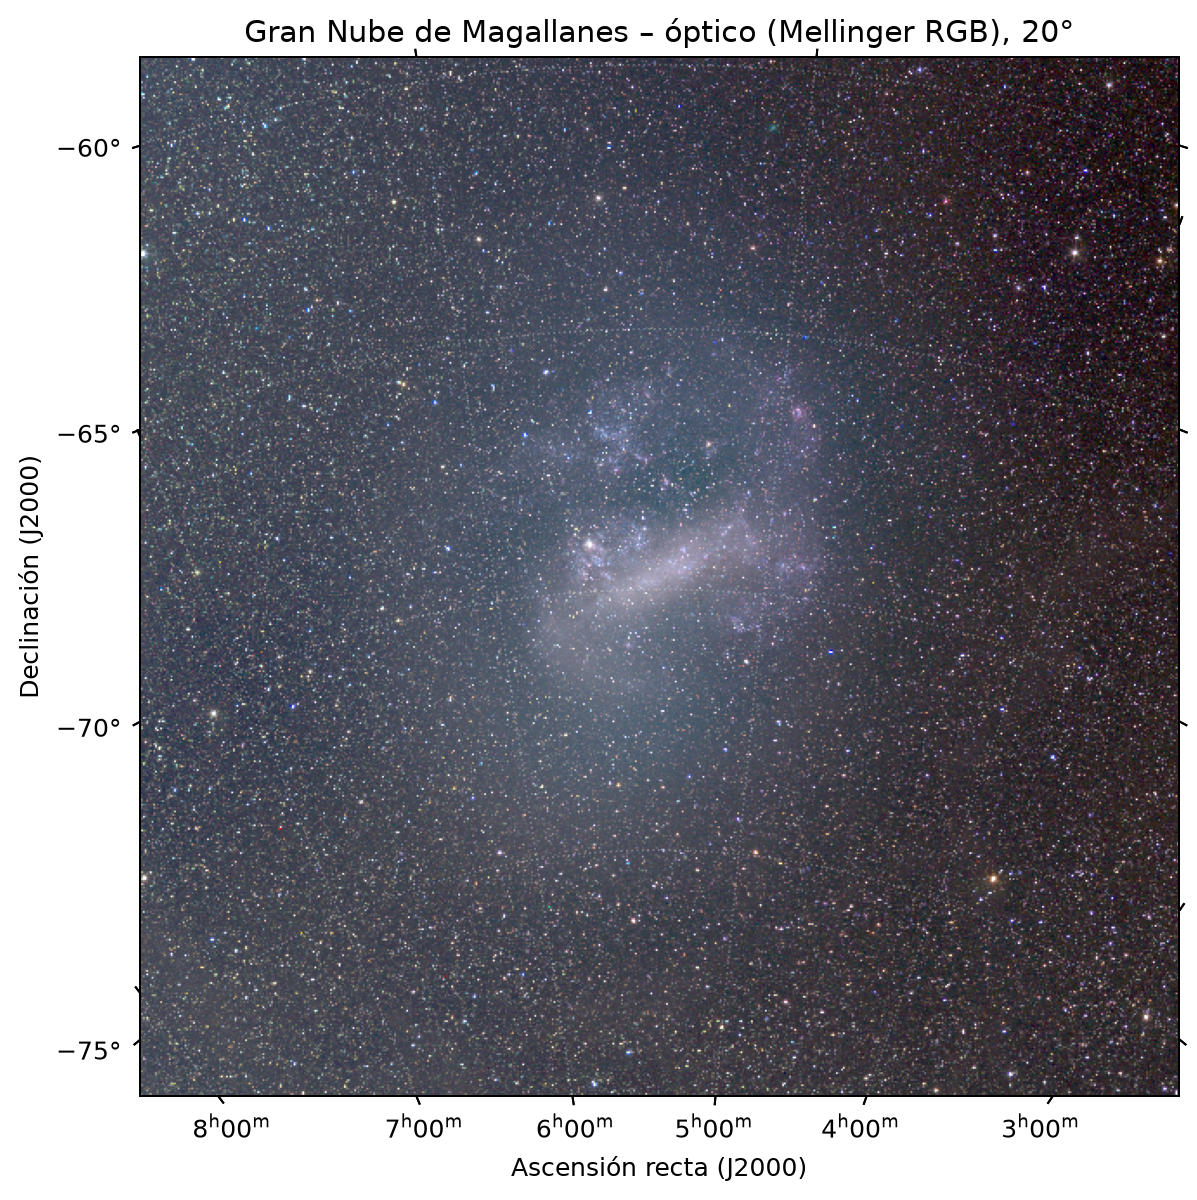
\includegraphics[width=0.42\textwidth]{punto4/LMC_optico_Mellinger_color_20deg.png}
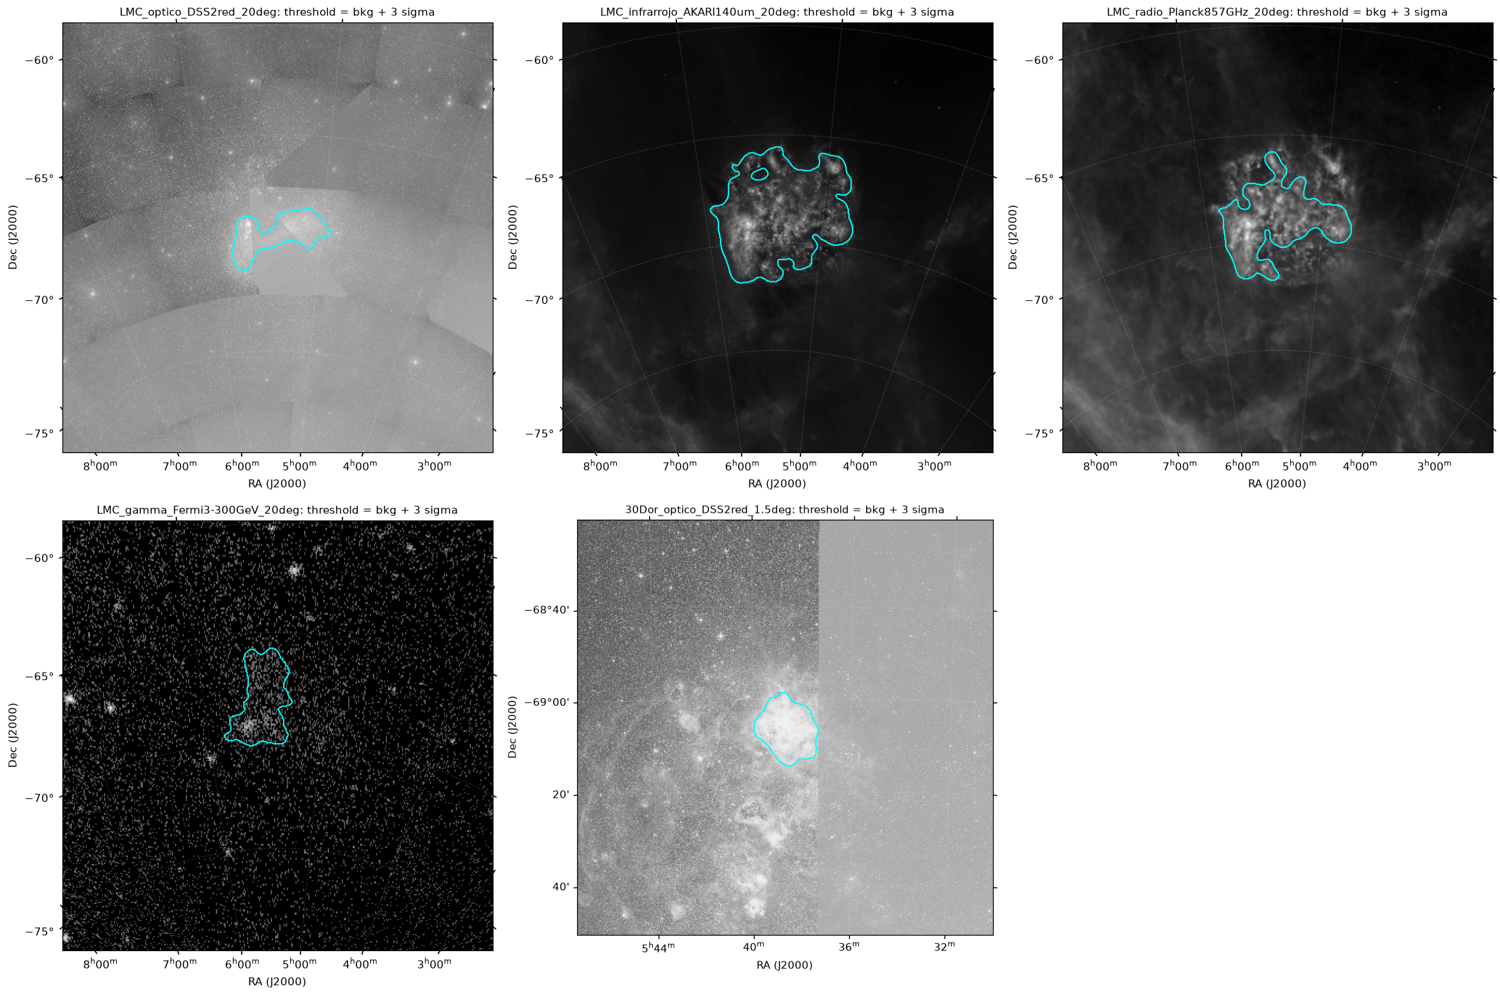
\includegraphics[width=0.56\textwidth]{punto4/panel_medidas_umbral3.png}
\caption{Izquierda: la LMC en óptico (Mellinger, color). Se ve la barra central alargada y el disco
difuso. Derecha: medida automática a $3\sigma$ (contorno cian) en óptico, infrarrojo (AKARI
\SI{140}{\micro m}), submilimétrico (Planck \SI{857}{GHz}), radio (Planck \SI{30}{GHz}), rayos gamma
(Fermi \SIrange{3}{300}{GeV}, suavizado $\sigma = 0.5^\circ$) y 30~Doradus.}
\label{fig:bandas}
\end{figure}

\subsection{(a) Diámetro angular en cada banda}

\subsubsection{Método automático}
Se suaviza la imagen, se estiman el fondo y su ruido $\sigma$, se marcan los píxeles por encima de
fondo $+\,N\sigma$ ($N = 2, 3, 5$) y se mide la región conectada que contiene el centro. El diámetro
equivalente es $D = 2\sqrt{\text{área}/\pi}$, y los ejes son los de la elipse con los mismos momentos.

\begin{table}[H]
\centering
\caption{Medida automática del diámetro equivalente (y ejes a $3\sigma$).}
\begin{tabular}{lcccc}
\toprule
Banda & $2\sigma$ & $3\sigma$ & $5\sigma$ & Ejes a $3\sigma$ \\
\midrule
Óptico (Mellinger) & $4.45^\circ$ & $3.25^\circ$ & $1.78^\circ$ & $4.87^\circ \times 2.42^\circ$ \\
Infrarrojo AKARI & $6.50^\circ$ & $5.98^\circ$ & $4.92^\circ$ & $6.98^\circ \times 5.51^\circ$ \\
Submm Planck 857 GHz & $5.59^\circ$ & $4.51^\circ$ & $3.09^\circ$ & $6.14^\circ \times 4.54^\circ$ \\
Radio Planck 30 GHz & $6.17^\circ$ & $5.11^\circ$ & $3.78^\circ$ & $5.66^\circ \times 5.39^\circ$ \\
Gamma Fermi ($\sigma = 0.5^\circ$) & $5.18^\circ$ & $3.86^\circ$ & $2.97^\circ$ & $5.10^\circ \times 3.08^\circ$ \\
30 Doradus & $15.8'$ & $13.7'$ & $9.0'$ & $15.5' \times 12.4'$ \\
\bottomrule
\end{tabular}
\end{table}

\subsubsection{Medida con regla}
Como comprobación independiente se imitó la herramienta de distancia de Aladin. A lo largo de cada
eje se calculó el perfil de brillo (mediana a través de una franja, sin suavizado 2D), y el borde se
puso donde el brillo cae al cielo vecino más un 10\,\% del contraste entre el pico y el cielo. Este
criterio se fijó antes de ver los resultados; 5\,\% y 20\,\% se usan como sensibilidad. Las reglas se
dibujaron en Aladin Desktop (figura~\ref{fig:reglas}).

\begin{table}[H]
\centering
\caption{Medida con regla frente a la automática y a los catálogos.}
\begin{tabular}{lcccc}
\toprule
Banda & Regla (10\,\%) & Rango 5--20\,\% & Automática $3\sigma$ & Referencia \\
\midrule
Óptico & $11.33^\circ \times 8.27^\circ$ & $7.5$--$13.1^\circ$ & $4.87^\circ \times 2.42^\circ$ & RC3: $10.76^\circ \times 9.16^\circ$ \\
AKARI & $6.43^\circ \times 4.80^\circ$ & $5.2$--$6.7^\circ$ & $6.98^\circ \times 5.51^\circ$ & -- \\
Planck 857 GHz & $6.53^\circ \times 4.03^{\circ\,\dagger}$ & $3.3$--$6.8^\circ$ & $6.14^\circ \times 4.54^\circ$ & -- \\
Planck 30 GHz & $7.10^\circ \times 5.60^\circ$ & $4.4$--$11.7^\circ$ & $5.66^\circ \times 5.39^\circ$ & -- \\
Fermi (mapa crudo) & no medible & -- & -- & -- \\
30 Doradus & $37.5' \times 30.0'$ & $23.9$--$47.1'$ & $15.5' \times 12.4'$ & SIMBAD: $40' \times 25'$ \\
\bottomrule
\multicolumn{5}{l}{\footnotesize $^\dagger$ No confiable: el borde se cortó en un hueco interno por los cirros de la Vía Láctea.}
\end{tabular}
\end{table}

\begin{figure}[htbp]
\centering
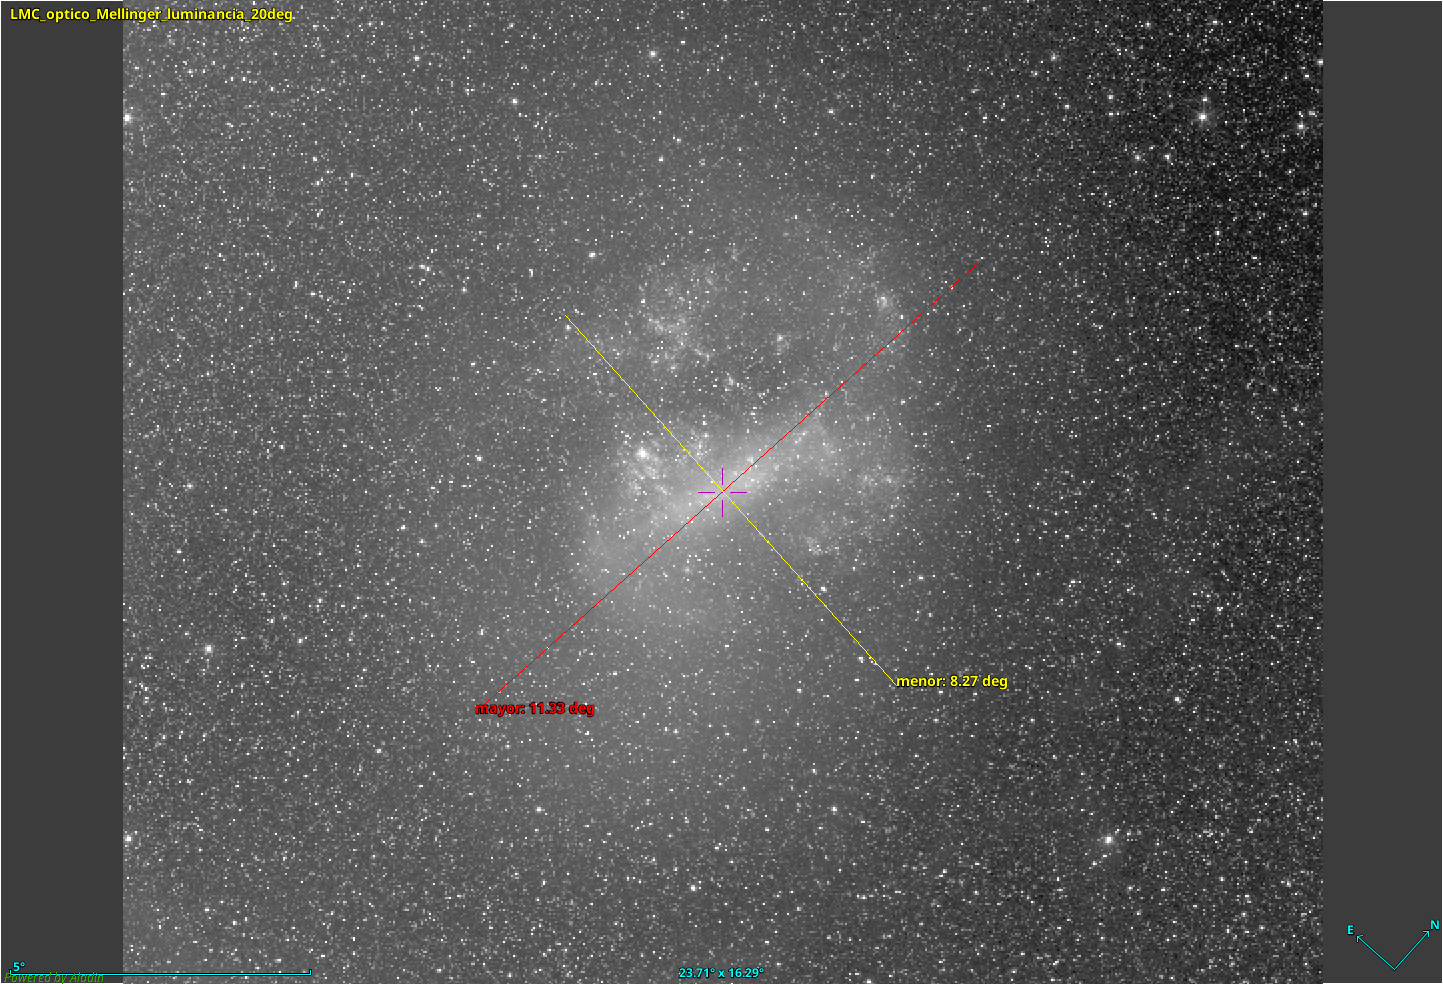
\includegraphics[width=0.32\textwidth]{capturas/aladin_regla_optico.png}
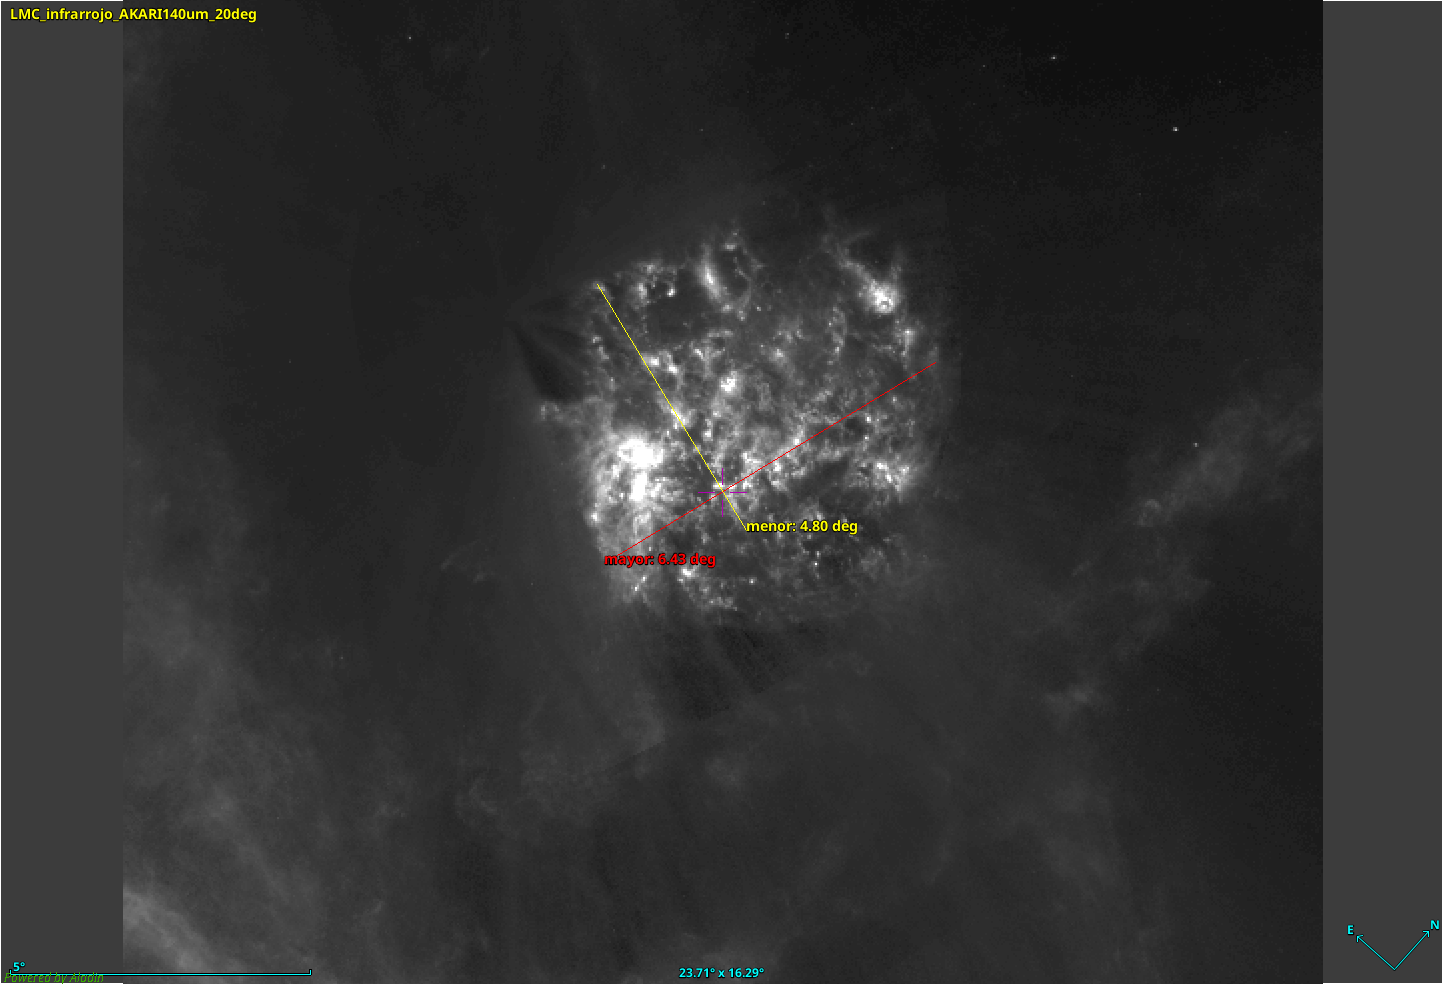
\includegraphics[width=0.32\textwidth]{capturas/aladin_regla_akari.png}
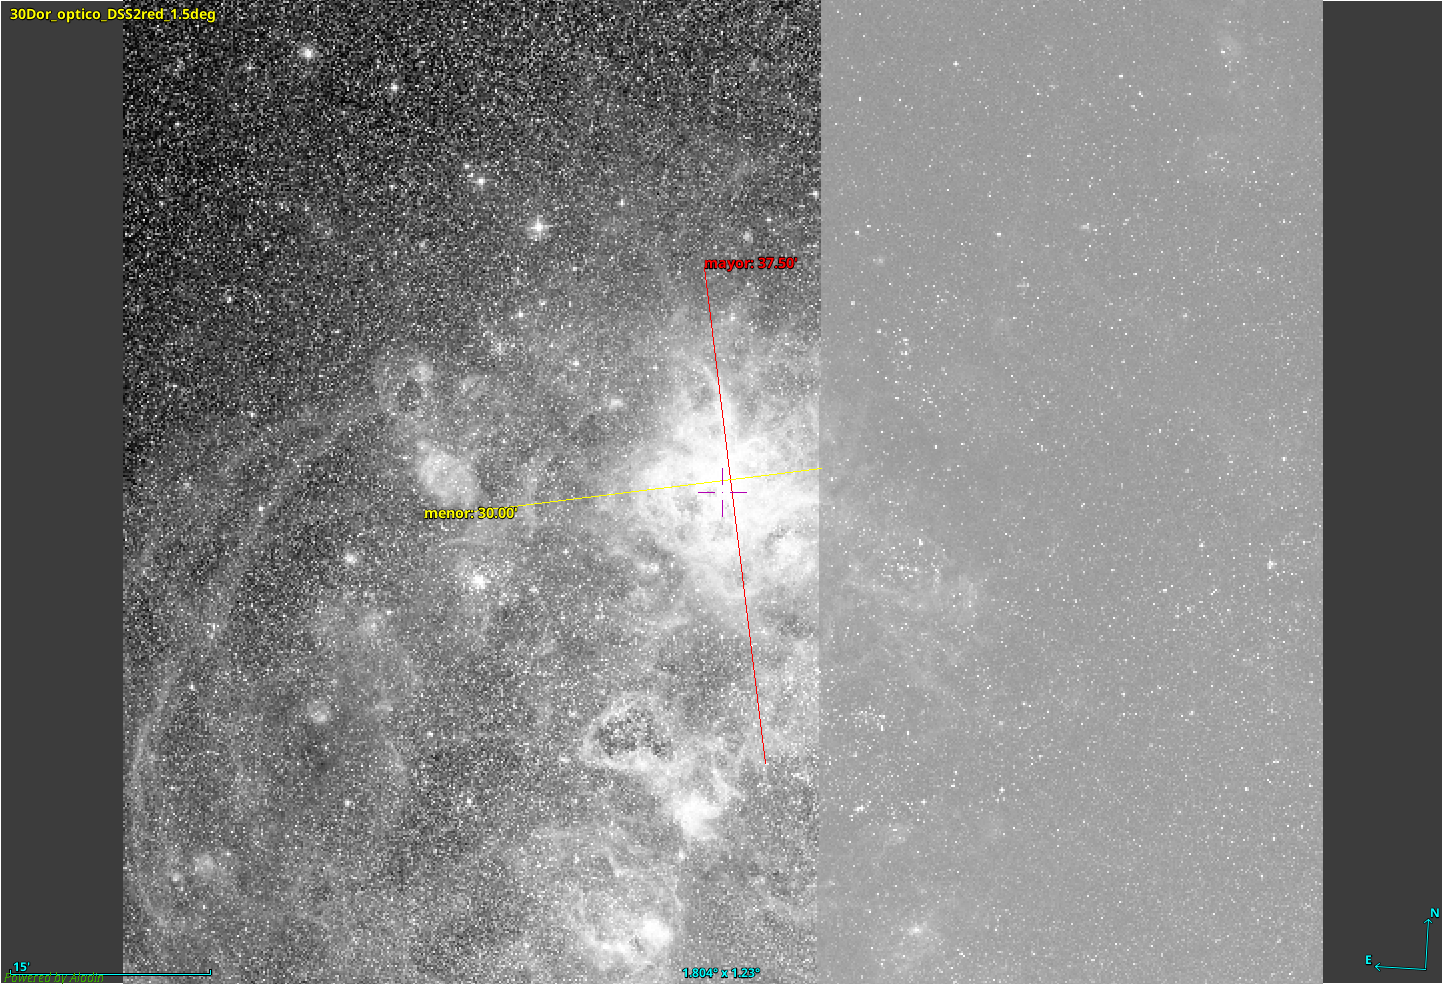
\includegraphics[width=0.32\textwidth]{capturas/aladin_regla_30dor.png}
\caption{Reglas dibujadas en Aladin Desktop (rojo: eje mayor; amarillo: eje menor) sobre el óptico,
el infrarrojo y 30~Doradus.}
\label{fig:reglas}
\end{figure}

\textbf{Resultados.} En las bandas con bordes nítidos (AKARI, Planck 857) los dos métodos coinciden
dentro del 8\,\%. En el óptico y en 30~Doradus la regla da más del doble que el método automático y
coincide con los catálogos: el umbral de $3\sigma$ corta el halo débil (el disco externo de la LMC, los
filamentos de la nebulosa) y deja solo la barra o el núcleo. En el mapa crudo de Fermi no hay borde;
para ver la LMC en rayos gamma hay que suavizar, y entonces el diámetro es una cota superior.

\subsubsection{Tamaño físico}
Con la aproximación de ángulo pequeño, $D = d\,\theta$ con $\theta$ en radianes y $d = \SI{50}{kpc}$:
\begin{table}[H]
\centering
\caption{Tamaño físico correspondiente.}
\begin{tabular}{lccc}
\toprule
Objeto & $\theta$ & $\theta$ (rad) & $D = \SI{50}{kpc}\cdot\theta$ \\
\midrule
LMC, óptico con regla (eje mayor) & $11.33^\circ$ & 0.1977 & \SI{9.9}{kpc} \\
LMC, RC3 (eje mayor) & $10.76^\circ$ & 0.1878 & \SI{9.4}{kpc} \\
LMC, AKARI automática $3\sigma$ & $5.98^\circ$ & 0.1044 & \SI{5.2}{kpc} \\
LMC, SIMBAD (eje mayor) & $5.38^\circ$ & 0.0939 & \SI{4.7}{kpc} \\
30 Doradus, regla (eje mayor) & $37.5'$ & 0.01091 & \SI{0.55}{kpc} \\
30 Doradus, SIMBAD & $40'$ & 0.01164 & \SI{0.58}{kpc} \\
\bottomrule
\end{tabular}
\end{table}

\subsubsection{¿Por qué cambia el tamaño con la longitud de onda?}
Cada banda ve un componente distinto. En \textbf{óptico} se ve la luz de las estrellas, con la barra
dominante y un disco externo débil. En el \textbf{infrarrojo lejano} (AKARI) se ve el polvo frío
calentado por estrellas jóvenes, repartido por todo el disco. En el \textbf{submilimétrico} (Planck
\SI{857}{GHz}) se ve polvo aún más frío, mezclado con cirros de nuestra galaxia. En \textbf{radio}
(Planck \SI{30}{GHz}) se ve el gas ionizado y los electrones relativistas, concentrados en las regiones
de formación estelar como 30~Doradus. En \textbf{rayos gamma} (Fermi) se ven los rayos cósmicos que
chocan con el gas; hay pocos fotones y la resolución es mala. No existe un único ``diámetro de la
LMC'': depende del componente y del criterio de borde.

\subsection{(b) Estrellas masivas de Bonanos et al.\ (2009)}
La tabla~3 de Bonanos et al.\ \cite{bonanos} (VizieR J/AJ/138/1003) da fotometría de 1268 estrellas
masivas. No trae una columna B$-$V: se calcula como $\text{Bmag} - \text{Vmag}$ (1135 estrellas con
ambas). Hay 35 estrellas (3\,\%) con $B-V < -0.5$ o $> 2.5$, físicamente imposibles (el color
intrínseco más azul es $\approx -0.33$; el margen hasta $-0.5$ cubre los errores fotométricos, de
mediana $0.05$--$0.07$~mag). Se marcaron y se graficaron aparte, sin borrarlas. Los datos se exportaron
a CSV y a Excel con un gráfico de dispersión con el eje V invertido.

\begin{figure}[htbp]
\centering
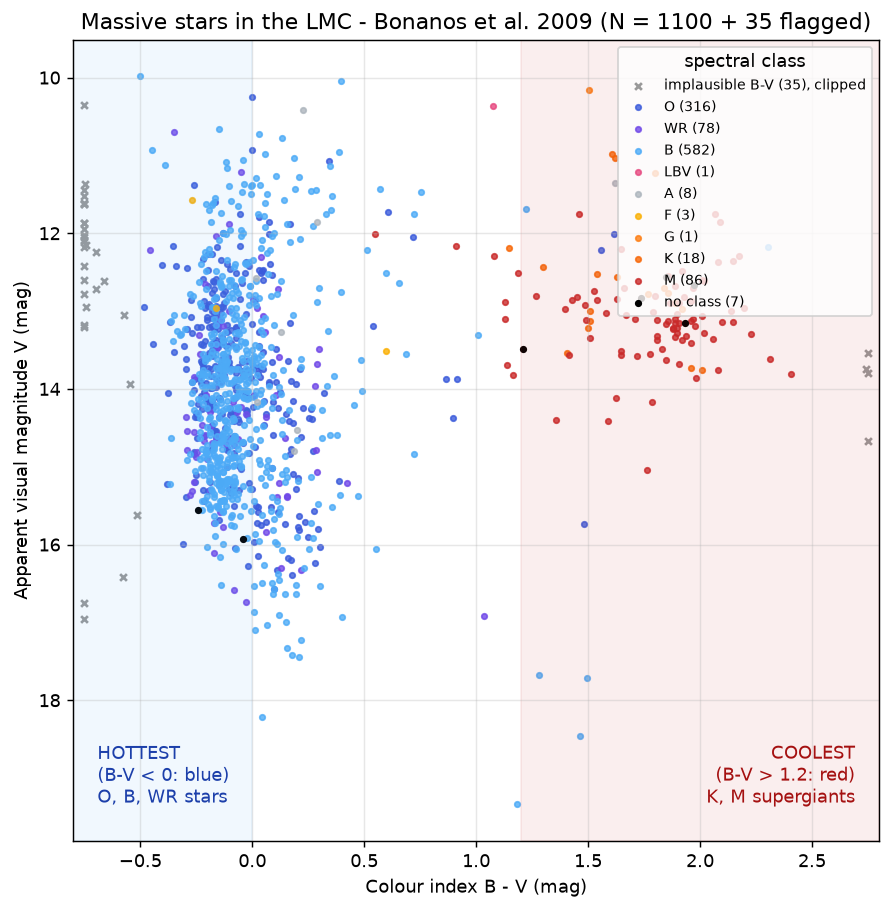
\includegraphics[width=0.49\textwidth]{punto4/Bonanos2009_LMC_V_vs_BV.png}
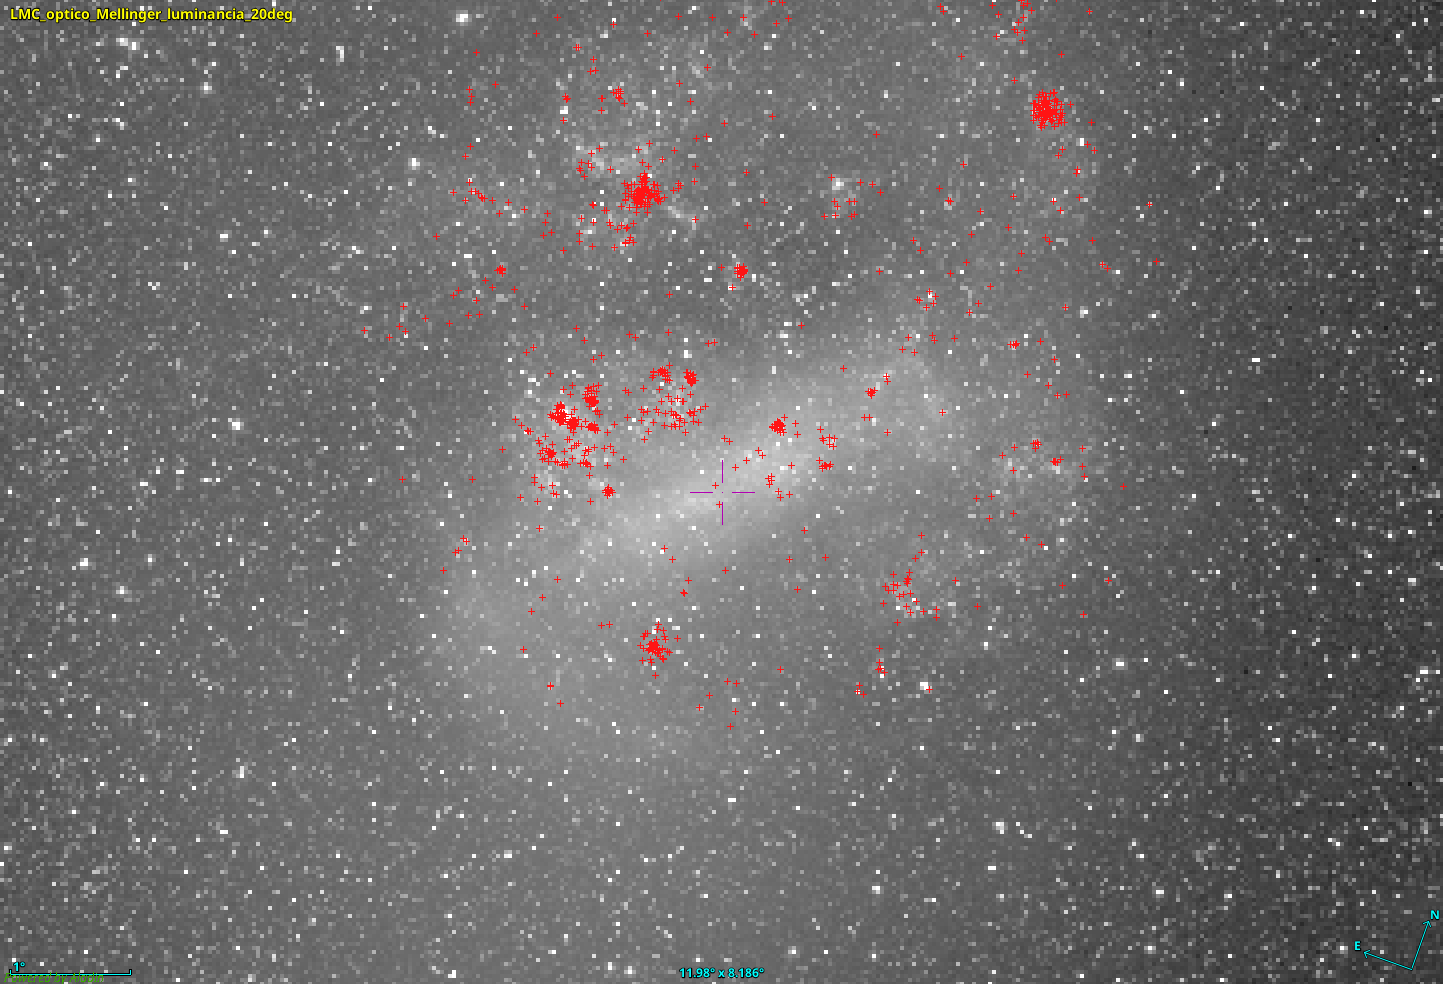
\includegraphics[width=0.49\textwidth]{capturas/aladin_Bonanos2009_sobre_LMC.png}
\caption{Izquierda: magnitud visual aparente V (eje invertido) contra índice de color B$-$V para
1100 estrellas masivas de la LMC, coloreadas por clase espectral. Derecha: las mismas estrellas
superpuestas en Aladin sobre la imagen óptica; se concentran en la barra y en 30~Doradus.}
\label{fig:cmd}
\end{figure}

\subsection{(c) ¿Dónde están las estrellas más frías y las más calientes?}

\begin{table}[H]
\centering
\caption{Índice de color B$-$V por clase espectral (1100 estrellas).}
\begin{tabular}{lccc}
\toprule
Clase & N & B$-$V medio & Rango \\
\midrule
O & 316 & $-0.05$ & $-0.48$ a $1.62$ \\
Wolf-Rayet & 78 & $-0.06$ & $-0.46$ a $1.03$ \\
B & 582 & $-0.03$ & $-0.50$ a $2.30$ \\
LBV & 1 & $+1.07$ & -- \\
A & 8 & $+0.34$ & $0.02$ a $1.62$ \\
F & 3 & $+0.06$ & $-0.27$ a $0.60$ \\
G & 1 & $+1.50$ & -- \\
K & 18 & $+1.66$ & $1.15$ a $2.01$ \\
M & 86 & $+1.76$ & $0.55$ a $2.41$ \\
Sin clase & 7 & $+1.20$ & $-0.24$ a $1.97$ \\
\midrule
Total & 1100 & & \\
\bottomrule
\end{tabular}
\end{table}

\textbf{a) Las más frías están a la derecha} del diagrama ($B-V$ entre $+1.2$ y $+2.4$): son
supergigantes rojas K y M, con superficies de unos \SIrange{3500}{4500}{K}. Están arriba, igual de
brillantes que las azules, porque son enormes.

\textbf{b) Las más calientes están a la izquierda} ($B-V \approx 0$ o negativo): estrellas O, B
tempranas y Wolf-Rayet, de \SI{20000}{K} a más de \SI{40000}{K}, entre ellas supergigantes azules.

\textbf{¿Por qué?} B mide el brillo en luz azul (\SI{\sim 440}{nm}) y V en luz visual
(\SI{\sim 550}{nm}). Por la ley de Wien, $\lambda_\text{máx} = b/T$ con
$b = \SI{2.898e-3}{m.K}$: una estrella de \SI{30000}{K} tiene su máximo en \SI{97}{nm}
(ultravioleta) y brilla más en B que en V, así que $B-V<0$. Una de \SI{3500}{K} tiene su máximo en
\SI{828}{nm} y brilla mucho más en V, así que $B-V$ es grande. Como todas están a la misma distancia
(módulo de distancia $m - M = 5\log_{10}(5000) = 18.5$), el eje V también ordena por luminosidad.

\textbf{Enrojecimiento.} El polvo absorbe más el azul que el rojo y aumenta $B-V$. Las estrellas O
deberían estar en $(B-V)_0 \approx -0.3$, pero su promedio observado es $-0.05$: un exceso de color
$E(B-V) \approx 0.25$~mag, debido al polvo de la Vía Láctea y al de la propia LMC.

% =====================================================================
\section{Punto 5: la edad de la Caja de Joyas (NGC 4755)}

\subsection{Datos de SIMBAD y de la literatura}
NGC~4755 es un cúmulo abierto en $12^\text{h}53^\text{m}39.6^\text{s}$, $-60^\circ22'16''$ (Cruz del
Sur), de $10.3'$ de tamaño, con paralaje $0.462 \pm 0.002$~mas y distancias publicadas de
\SIrange{1.89}{1.99}{kpc}. Su edad, según tres estudios independientes, es de
$10 \pm 5$~Ma \cite{sanner}, $14 \pm 2$~Ma \cite{bonatto} y 16~Ma \cite{piskunov}.

\begin{table}[H]
\centering
\caption{Estrellas más brillantes del cúmulo (SIMBAD).}
\begin{tabular}{llcc}
\toprule
Estrella & Tipo espectral & V & B$-$V \\
\midrule
HD 111904 & B9\,Iab (supergigante azul) & 5.77 & 0.28 \\
$\kappa$ Cru & B5\,I (supergigante azul) & 5.94 & 0.18 \\
HD 111990 & B1.5\,I (supergigante azul) & 6.78 & 0.17 \\
BU Cru & B2\,Ib (supergigante azul) & 6.84 & 0.20 \\
DU Cru & M2\,Iab (supergigante roja) & 7.66 & 2.16 \\
CC Cru & B2\,III (gigante azul) & 7.83 & 0.17 \\
\bottomrule
\end{tabular}
\end{table}

\begin{figure}[htbp]
\centering
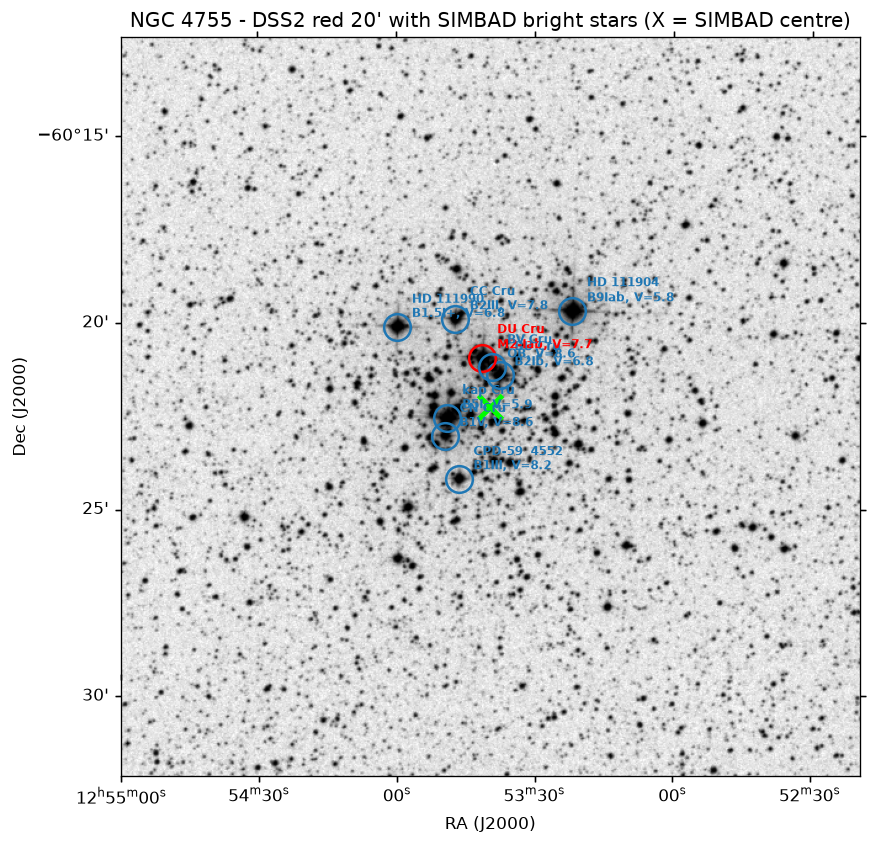
\includegraphics[width=0.48\textwidth]{punto5/NGC4755_DSS2red_estrellas_identificadas.png}
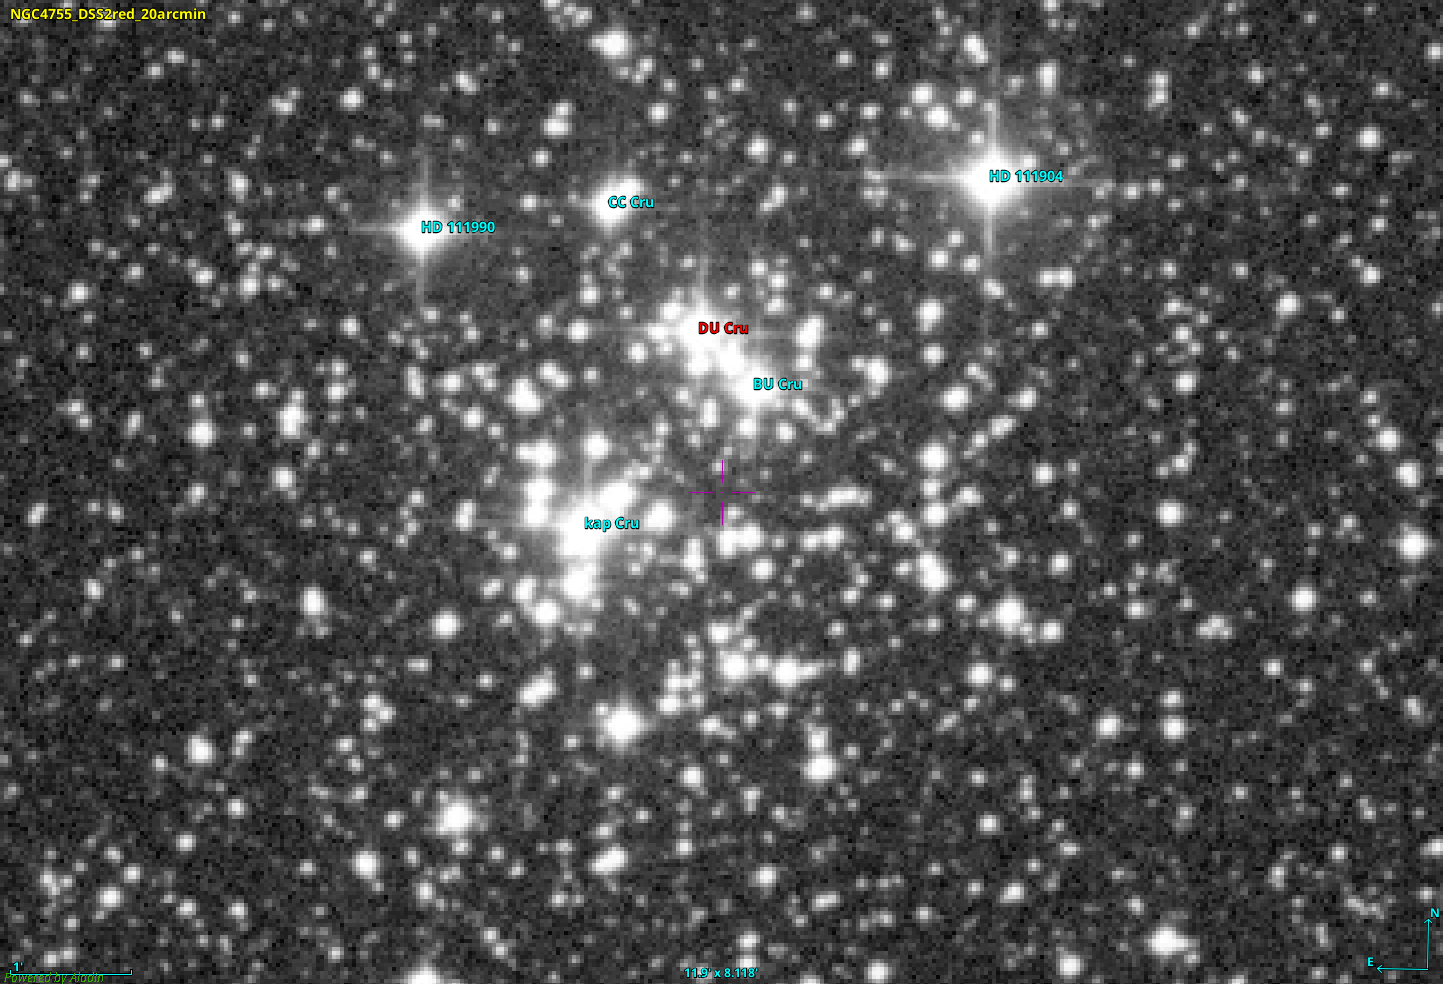
\includegraphics[width=0.48\textwidth]{capturas/aladin_NGC4755.png}
\caption{NGC~4755 en DSS2 roja con las estrellas de SIMBAD identificadas (izquierda) y la misma
región en Aladin (derecha). La orientación coincide con la foto del taller: la estrella naranja de
la foto es DU~Cru.}
\end{figure}

\subsection{(1) Centro, límite y estimación de brillo y color}
El centro (X) se puso en el baricentro de las tres concentraciones brillantes del núcleo: DU~Cru, BU~Cru
y el grupo de $\kappa$~Cru. Coincide con el centro de SIMBAD y con el máximo de densidad de estrellas
de la foto. El límite visible en la foto ($\approx 6'$ de cielo) es el del núcleo, no el del cúmulo
completo ($10.3'$). Dentro de un cuadrado de unos $2'$ de lado se estimaron el color (por el halo de
cada estrella, comparado con la barra O$\ldots$M) y el brillo (por el tamaño del punto, escala 1--10).

\begin{table}[H]
\centering
\caption{Estrellas dentro del cuadrado por brillo y color (46 en total).}
\begin{tabular}{ccccccccccc}
\toprule
Brillo & O & B & A & F1 & F2 & G & K1 & K2 & M \\
\midrule
2 & & & & & & & & 1 & \\
3 & & 1 & & & & & & & \\
4 & & & 1 & & & & & & \\
5 & & 5 & 2 & & & & & & \\
6 & & 2 & 1 & & 1 & & & 1 & \\
7 & & 3 & 7 & 7 & 1 & & 1 & & \\
8 & & & 3 & 8 & 1 & & & & \\
\bottomrule
\end{tabular}
\end{table}

\begin{figure}[htbp]
\centering
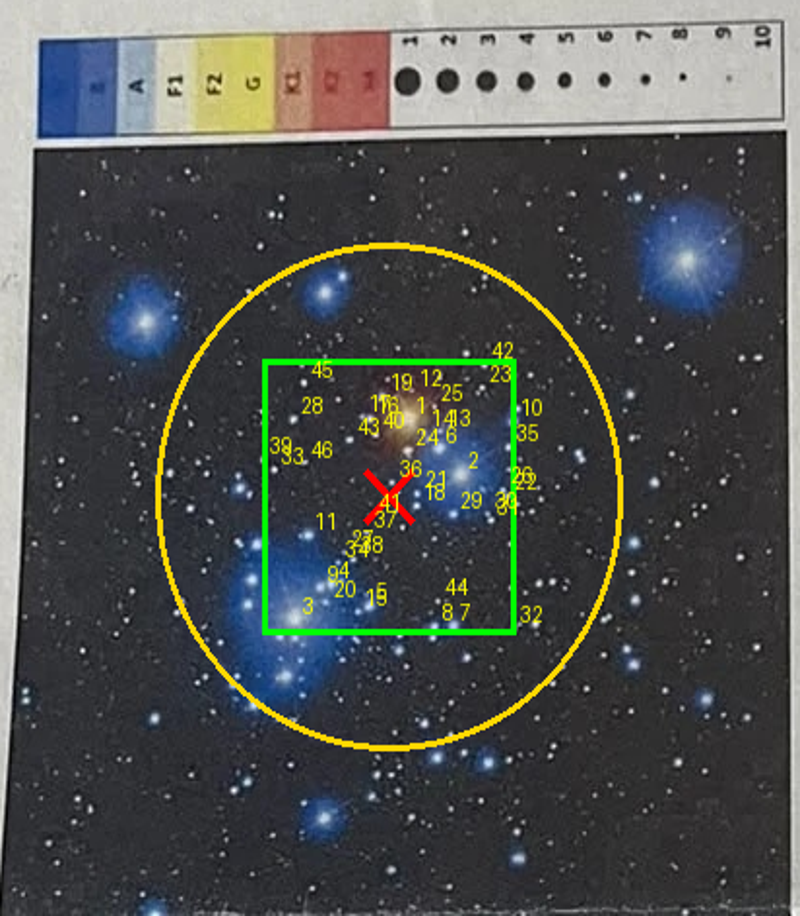
\includegraphics[width=0.40\textwidth]{punto5/pagina2_cumulo_ampliado.png}
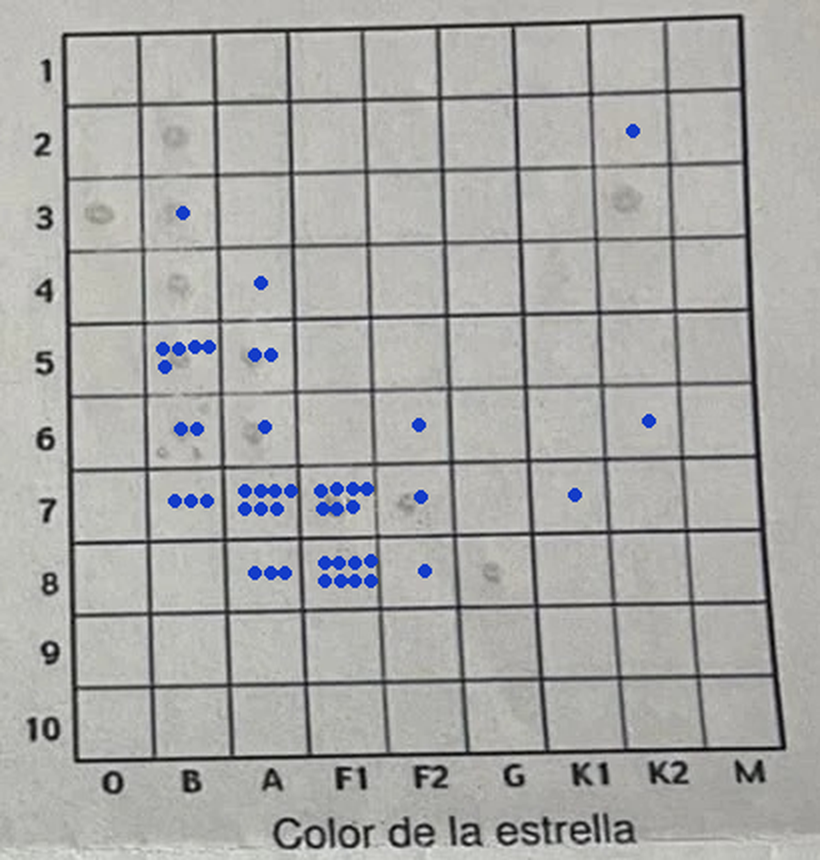
\includegraphics[width=0.40\textwidth]{punto5/hoja_de_trabajo_sobre_la_foto_ampliada.png}
\caption{Izquierda: la foto del taller con el centro (X roja), el límite (círculo amarillo) y el
cuadrado de muestreo (verde). Derecha: la hoja de trabajo con las estimaciones (puntos azules).}
\label{fig:hoja}
\end{figure}

\subsection{(2) Estimación de la edad}
En los diagramas de referencia, un cúmulo \textbf{joven} ($< 100$~Ma) tiene estrellas azules muy
brillantes arriba a la izquierda; uno de \textbf{edad intermedia} (100--3000~Ma) ya no las tiene y
muestra gigantes rojas; uno \textbf{viejo} ($> 3000$~Ma) solo conserva la parte baja de la secuencia
y muchas gigantes rojas. La hoja de trabajo (figura~\ref{fig:hoja}) muestra estrellas B brillantes
arriba a la izquierda, una secuencia que baja hacia A y F, y una sola estrella roja muy brillante
(DU~Cru). \textbf{La Caja de Joyas es un cúmulo joven.}

\begin{figure}[htbp]
\centering
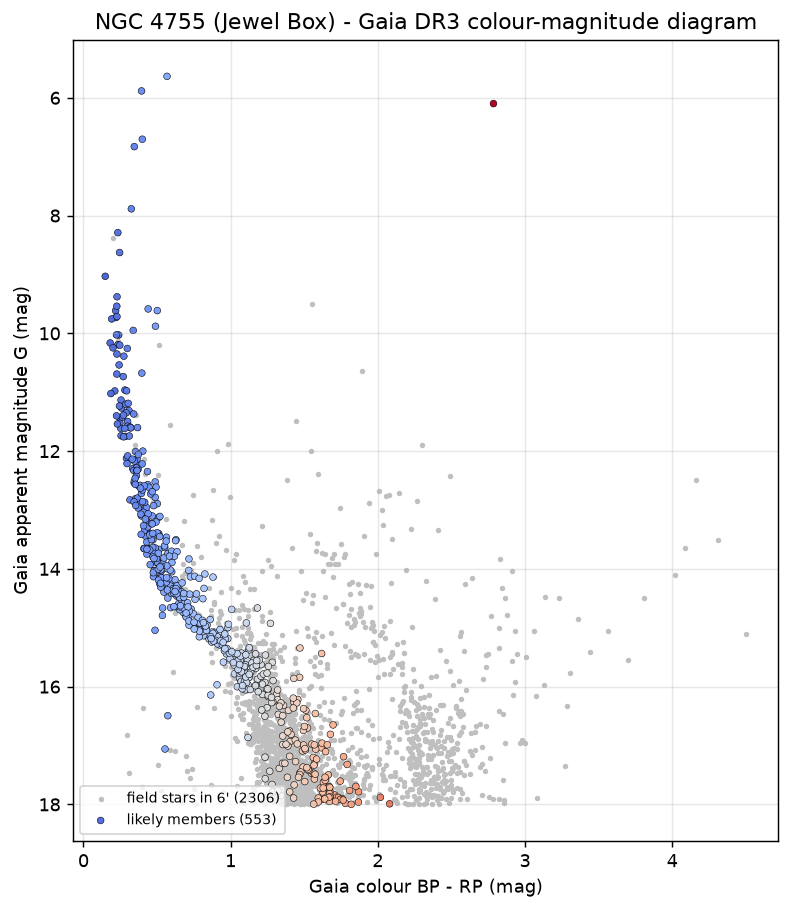
\includegraphics[width=0.62\textwidth]{punto5/NGC4755_GaiaDR3_CMD.png}
\caption{Diagrama color-magnitud real de NGC~4755 con Gaia DR3: 553 miembros probables (paralaje
$0.470$~mas, movimiento propio común $\mu_{\alpha*} = -4.71$, $\mu_\delta = -1.08$~mas/año) entre 2306
estrellas en un radio de $6'$. El recuadro verde marca el punto de giro.}
\label{fig:gaia}
\end{figure}

El diagrama de Gaia (figura~\ref{fig:gaia}) lo confirma. La secuencia principal sube casi vertical
($BP-RP \approx 0.23$). Las cuatro estrellas azules más brillantes ($G = 5.6$--$6.8$) están corridas a
la derecha ($BP-RP = 0.35$--$0.57$): son las estrellas B más masivas, que ya salen de la secuencia
principal. Hay además una única supergigante roja (DU~Cru). Que el punto de giro esté en estrellas B
tan masivas indica una edad de unos 10 a 15 millones de años, de acuerdo con la literatura.

% =====================================================================
\appendix
\section{Fuentes de datos y herramientas}\label{ap:fuentes}
Los servidores del CDS (SIMBAD, VizieR y Aladin/hips2fits en Estrasburgo) no respondieron durante todo
el trabajo, incluso desde dos redes distintas. Se usaron:
\begin{itemize}
  \item SIMBAD a través de su espejo de Harvard (\texttt{simbad.harvard.edu}).
  \item Imágenes de NASA SkyView: Mellinger (rojo, verde y azul), AKARI WIDE-L, Planck
  \SI{857}{GHz} y \SI{30}{GHz}, Fermi (bandas 1 a 5) y DSS2 roja.
  \item La tabla~3 de Bonanos et al.\ (2009) en formato legible por máquina, publicada por la revista.
  \item Gaia DR3 desde el archivo de la ESA, y RC3 a través de NED.
\end{itemize}
Las consultas, descargas, medidas y figuras se hicieron con un servidor MCP propio
(\texttt{aladin-mcp}) y scripts en Python (astropy, astroquery), y Aladin Desktop se controló por
SAMP. Todo el código y los datos están en
\url{https://github.com/sebastianvelace/aladin-mcp}.

\sloppy
\begin{thebibliography}{9}
\bibitem{bonanos} A.~Z. Bonanos et al., \emph{Spitzer SAGE infrared photometry of massive stars in the
Large Magellanic Cloud}, AJ \textbf{138}, 1003 (2009).
\bibitem{sanner} J.~Sanner, J.~Brunzendorf, J.-M. Will y M.~Geffert, \emph{Photometric and kinematic
studies of open star clusters. III. NGC 4103, NGC 5281, and NGC 4755}, A\&A \textbf{369}, 511 (2001).
\bibitem{bonatto} C.~Bonatto, E.~Bica, S.~Ortolani y B.~Barbuy, \emph{Detection of Ks-excess stars in
the 14 Myr open cluster NGC 4755}, A\&A \textbf{453}, 121 (2006).
\bibitem{piskunov} A.~E. Piskunov et al., \emph{On the determination of age and mass functions of stars
in young open star clusters from the analysis of their luminosity functions}, MNRAS \textbf{349}, 1449
(2004).
\bibitem{rc3} G.~de Vaucouleurs et al., \emph{Third Reference Catalogue of Bright Galaxies} (RC3), 1991.
\bibitem{simbadlmc} Tamaño óptico de la LMC en SIMBAD, referencia 2014MNRAS.445..881C.
\bibitem{naoj} National Astronomical Observatory of Japan, \emph{Venus at greatest brilliancy} (2017).
\bibitem{earthsky} EarthSky, \emph{Venus at its brightest in the morning sky} (2026).
\end{thebibliography}

\end{document}
